\section{Example Autogenerated Prometheus Config}
\begin{listing}[H]
  \inputminted{yaml}{./prom.yml}
\caption{Example Autogenerated Prometheus Config (target list truncated and reformatted)}
\end{listing}
\section{Prometheus Node Utilization data}
All data was collected by running \texttt{vmstat} each second while running the benchmarks

\subsection{I/O was not the bottleneck}
\begin{figure}[H]
  \centering
  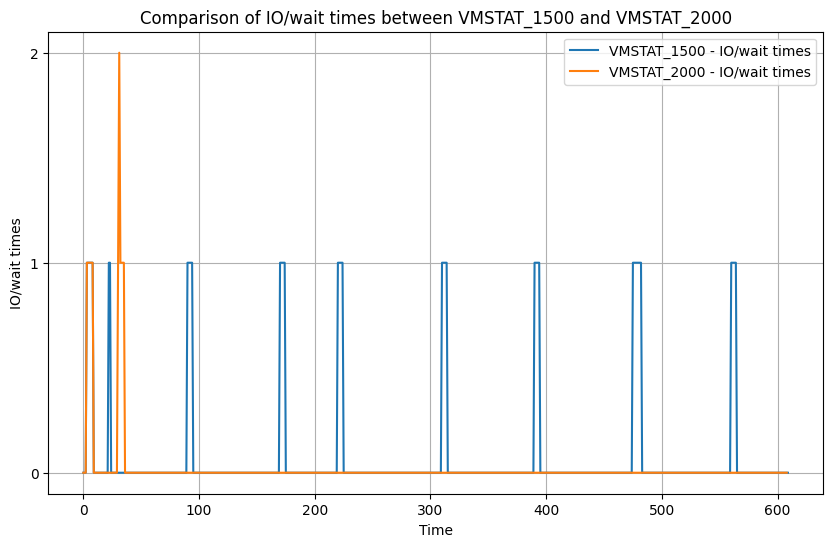
\includegraphics[width=\textwidth]{./plots/p1_iowait.png}
  \caption{The I/O wait times recorded, showing that there was no increasing queue of I/O operations.}
\end{figure}

\subsection{Memory was not the bottleneck}

\begin{figure}[H]
  \centering
  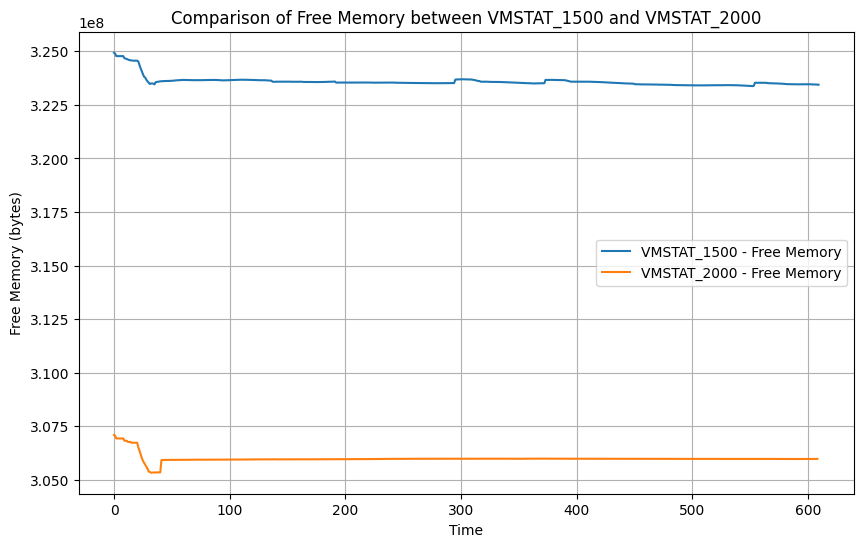
\includegraphics[width=\textwidth]{./plots/p1_freemem.png}
  \caption{The free memory, showing that there was more than enough free memory, and that the memory usage was not significantly different between the benchmarks.}
\end{figure}

\begin{figure}[H]
  \centering
  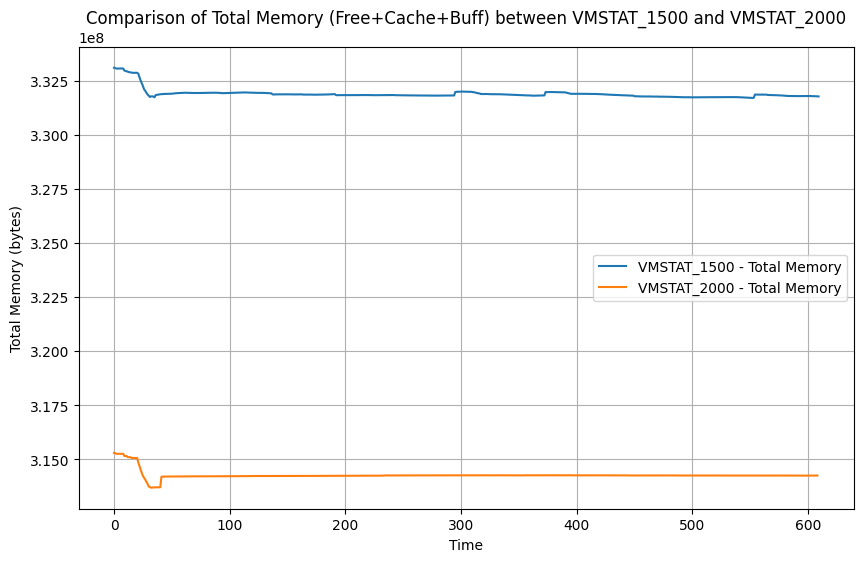
\includegraphics[width=\textwidth]{./plots/p1_totalmem.png}
  \caption{The total non-used memory (including page cache and buffer cache), again showing no significant difference between the well performing 1500 node benchmark and the slow 2000 node benchmark}
\end{figure}

\begin{figure}[H]
  \centering
  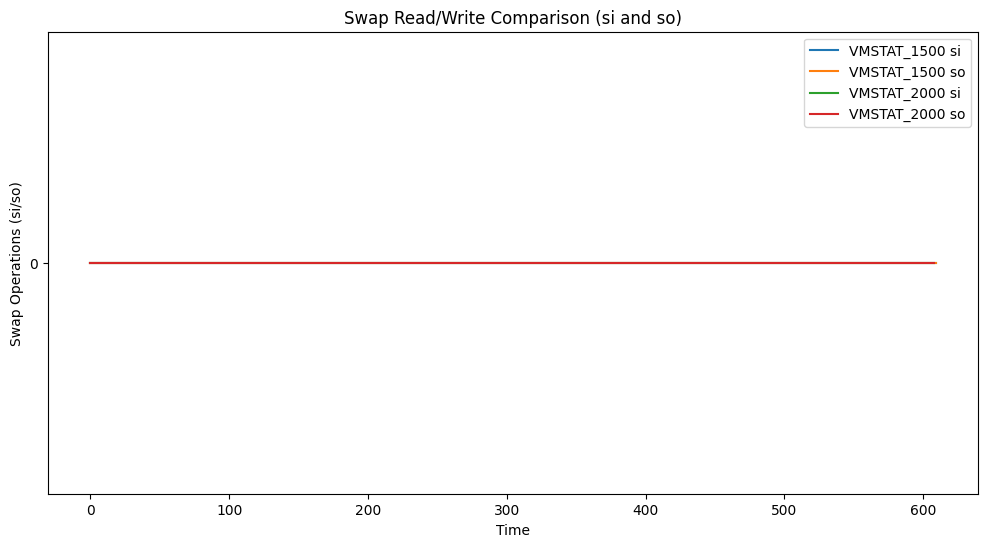
\includegraphics[width=\textwidth]{./plots/p1_swapio.png}
  \caption{No swap was used at both benchmarks.}
\end{figure}

\subsection{CPU was not the bottleneck}

\begin{figure}[H]
  \centering
  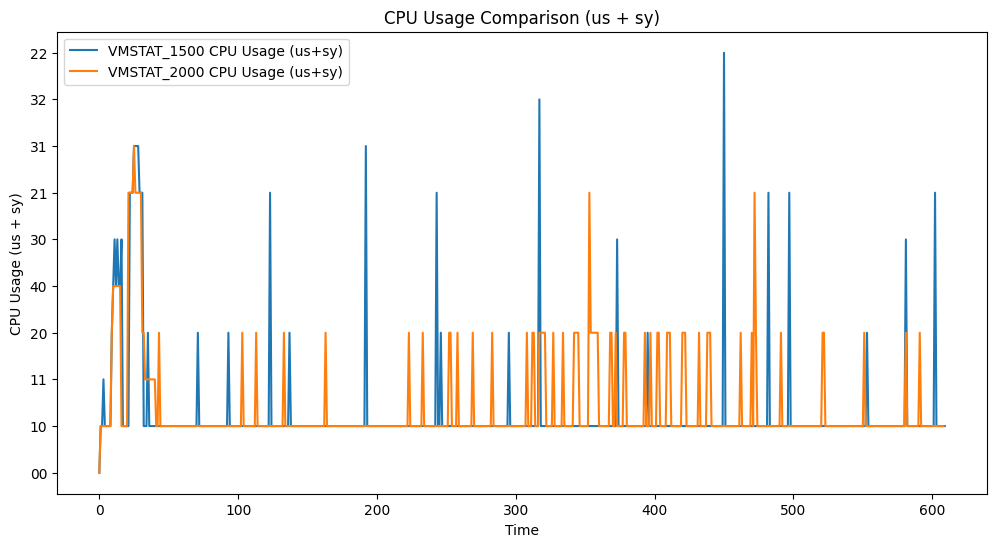
\includegraphics[width=\textwidth]{./plots/p1_cpu.png}
  \caption{The accumulated CPU usage, both system time (sy) and user time (us), showing that the processor was not fully utilized in both benchmarks, and that due to the high amount of threads available the CPU usage was not significantly different.}
\end{figure}
